\chapter{Background}\label{chp:background}

Creating and maintaining real-world knowledge bases in a classical work environment demands a high cost, and is a cost that is often unnecessary [\citep{Meier2013}, p. 134]. Alternative approaches are to rely on the knowledge of open crowds, volunteer contributions, or services like micro-tasking platforms where there are people ready to work on the tasks given to them [\citep{Meier2013}, p. 134].   

Today, geospatial data is more available than ever. Governments are releasing more and more data and the OpenStreetMap database is still growing. While general data availability is increasing, the quality of the data is not necessarily perfect and manual pre-processing is often necessary before using it \citep{Difallah2015}.  Pre-processing of the data are time consuming and expensive. By exploiting both machines and people through the appropriate platform and approach, the cost can decrease and the quality increase. We will argue that combining machines and people is often a better and faster solution than a fully-automatic or fully-manual approach. Implementing this kind of approach into a micro-tasking platform can be a good solution. 

\section{Why do we need humans?}\label{sec:whyneedhumans}
%hvorfor kan man ikke bare bruke ai? Skrive et avsnitt 3 ai bedrifter har microtasking i scopet ditt, nevne dette i introen
%https://pdfs.semanticscholar.org/d23b/1e9285d1d4b487e504d728d023d779d0ae65.pdf
%"Machine learning" was originally defined as "... artificial generation of knowledge from experienced". The first machine-learning procedures could play the game of checkers. The computer could be programmed so that it learned to play a better game of checkers than by the person who wrote the program after only 8-10 hours of training \citep{Samuel1959}. 

Machine learning gives computers the ability to learn without being explicitly programmed. It involves computer intelligence, but the computers do not know the answers up front \citep{StanfordUniversity2017}. Machine-learning algorithms have enormous problems when contextual information is missing. Without a pre-set of rules, a machine has trouble solving the problem. Machines do not have creativity, which is required to answer complex problems \citep{Holzinger2016a}. According to the company Mighty AI\footnote{Mighty AI generates high-quality AI training data.}, humans cannot be removed from Artificial Intelligence training loops. Machine-learning approaches still require a huge amount of training data to work on new domains \citep{Schulze2012}. Mighty AI believe that humans will continue to play a crucial role in creating training data for the algorithms \citep{Gutzwiller2017}. %*Riktig å skrive algoritme her? kilde https://mty.ai/blog/why-you-cant-remove-humans-from-ai-training-loops/

It is suggested by \cite{Biewald2015} and \cite{Oppenheimer2017}  that machine learning accuracy should follow the Pareto 80:20 principle. Getting 80 \% accuracy can be reasonably easy to accomplish, but the last 20 \% should be handled by human input \citep{Biewald2015} \citep{Oppenheimer2017}. Important human input is providing training data and to route tasks when the algorithm is unsure of its answer [\citep{Oppenheimer2017}, \citep{Nakhuda2016}]. The machine learning company developmentSEED\footnote{DevelopmentSEED is a creative engineering team solving complex problems with open software and open data.} use a micro-tasking solution to clean their machine learning output data. They are using humans to get a faster, more accurate output data by developing Skynet Scrubber, a GUI web application solution to get human input quicker and easier \footnote{developmentSEED's algorithm is called Skynet}. In their blog, Derek Lieu writes: "Skynet gets more capable every day, but the output is still not perfect [..] We built Skynet Scrub so we could start using Skynet data sooner" \citep{Lieu2017a}. 

\cite{Holzinger2016} claim that most people from the machine learning community are concentrating on \textit{automatic} machine learning by bringing the humans out of the process. When humans are out of the loop, the training data sets can be uncertain and incomplete, and the resulting algorithm can be questionable \citep{Holzinger2016}. By bringing humans back in the process, especially in domains where the data sets are questionable, for instance in the health domain, one enables what neither a human or a computer can do on their own \citep{Holzinger2016}. It is possible to build hybrid human-machine systems that combine both the scalability of computers and the yet unmatched cognitive abilities of the human brain \citep{Difallah2016}. 
%reCaptcha is a good example of how to exploit human cognitive abilities. Humans are through this solution identifying themselves as a human, and at the same time digitizing old books. In older books where the pages are bleached and yellow, machines struggle to understand what the words say. 750 000 000 individuals have helped digitize books through reCaptcha. %https://www.youtube.com/watch?v=cQl6jUjFjp4
"Computers are bad at finding patterns unless we have a well-understood problem" \citep{Cohen2013}, who is the co-founder of Palantir Technologies \footnote{Palantir builds software that connects data, technologies, humans and environments}. Only humans can understand and frame a new problem. %https://www.youtube.com/watch?v=KvAXkA7u_A0
%Why Artificial Intelligence Needs a Task Theory + https://link.springer.com/chapter/10.1007/978-3-319-41649-6_12
Palantir Technologies believe in augmenting human intelligence, not replacing it. As \cite{Holzinger2013} say, "[...] the problem-solving knowledge is located in the human mind and - not in machines, " and this is something we must acknowledge. 

\section{Human computation}\label{sec:humancomputation}
%Problems computers cannot solve/struggle with (yet)
Human computing is, at its most general level, computation performed by human beings and a human computation system contains both humans and computers working together to solve difficult problems \citep{Schulze2012}. We argue that utilizing the human processing power is still important. Humans are necessary even though our computers are becoming more and more complex. Traditional approaches to solving problems are to focus on improving the software, but as the reader will see in this thesis, a solution that uses humans cleverly by exploiting the human brain cognitive abilities can create much faster and better results than software. One of the pioneers of crowdsourcing, Luis von Ahn, wanted to find a cheap and efficient way to label images \citep{VonAhn2008}. The solution was to exploit the use of a game-like approach in a non-game context to motivate individuals to label the pictures through a game. This approach is called gamification \citep{Huotari2017}. The game was called "The ESP game" and solved the problem of labeling images with words. Most images do not have a proper caption associated with them, and this makes it difficult to create search engines for images. A fast and cheap method of labeling images is by using humans cleverly, and humans can very easily see if the picture contains, i.e., a dog or a cat. Through "The ESP game" humans where labeling images without even knowing it, they only played a fun game. Within a few months, the game collected more than 40 million image labels \citep{VonAhn2008}, and they did not even have to pay them to do it. 
%Another game that was created by Luis Von Ahn is called "Peekaboom," this is also using a gamification approach. Here the players would locate objects in images. Such information is very useful in computer vision research for instance \citep{VonAhn2008}. 
Human computation is one of the major areas where the gamification approach has been employed \citep{Morschheuser2016}. Each human performs a small part of a massive computation task.  

\begin{figure}[H]
	\centering
	\includegraphics[width=0.4\linewidth]{../../../../../Desktop/humancomp_crowdsourcing}
	\caption{Collective intelligence \citep{Quinn2011}}
	\label{fig:humancompcrowdsourcing}
\end{figure}

Human computation, a term introduced by Luis von Ahn, refers to, according to \cite{Quinn2011}, a distributed system that combine the strengths of humans and computers to accomplish tasks that neither can do alone. To make human computation in crowdsourcing compelling one needs to know how the results can be optimally acquired from humans and how the results can be integrated into productive environments without having to change established workflows and practices [\citep{Meier2013}, p. 134]. Gamification can be one solution on how to make human computation in crowdsourcing effective \citep{Wang2017}. The author will argue that micro-tasking can be another solution for effective crowdsourcing using humans cognitive abilities.

\section{Crowdsourcing}\label{sec:crowdsourcing}
%What is it
The first time the term "crowdsourcing" appeared was in Wired magazine article by Jeff Howe \citep{Howe2006}. Whereas human computing (\ref{sec:humancomputation}) replaces computers with humans, crowdsourcing replaces traditional human workers with members of the public \citep{Quinn2011}. Crowdsourcing companies came onto the scene with the goal of helping businesses solve simple problems with massive scale \citep{Webster2016}. \cite{EYeka2015} state that 85 \% of the top global brands use crowdsourcing for various purposes. Crowdsourcing is an increasingly important concept \citep{Salk2016} and has become a widespread approach to dealing with machine-based computations where we leverage the human intelligence \citep{Gadiraju2015}. Crowdsourcing is a way of refactoring work in a way that exploits the worker's flexibility and gets the right skills to the right part of the problem. To get the right skills to the right part of the problem it needs to be partitioned into smaller parts. Having smaller parts will make it easier to distribute the problem. The distribution can be done through micro-tasking, also called "smart crowdsourcing" by Patrick Meier \citep{Meier2013a}. 

When the field of a crowdsourced project is explicitly geographical, it is often called \textit{volunteered geographical information} (VGI). According to \cite{Salk2016}, the best known VGI project is OpenStreetMap (OSM). OSM is an open-source mapping project, where volunteers contribute with their local knowledge and mapping abilities, called "the Wikipedia of maps" \citep{Palen2015}. Wikipedia can be said as being the best known and most successful example of crowdsourcing on a global scale. \cite{Chilton2009} suggested that the OSM project would have a similar impact on open and free geodata as Wikipedia had on 'fact finding'.

\section{Micro-tasking}\label{sec:microtasking}
%What is it
The simplest type of tasks are called micro-tasks and is illustrated in figure \ref{fig:microtaskingillustration}. Micro-tasks should not require any special training, and a task should be completed within a couple of minutes \citep{Ipeirotis2010}. Problems that are suitable for solving through micro-tasking are those that are easy to distribute into many simple tasks, which can be completed in parallel in a relatively short period of time, without requiring specific skills \citep{Sarasua2012}. Research has also demonstrated that micro-tasking is effective for far more complex problems when using sophisticated workflow management techniques. Micro-tasking can then be applied to a broader range of challenges like: 1) completing surveys, 2) translating text between two languages, 3) matching pictures of people, 4) summarizing text \citep{Bernstein2015a}. 

\begin{figure}[H]
	\centering
	\includegraphics[width=0.6\linewidth]{../../../../../Desktop/microtasking_illustration}
	\caption{Micro-tasking \citep{Michelucci2015}}
	\label{fig:microtaskingillustration}
\end{figure}

\subsection{Micro-tasking platforms}
It exists multiple micro-tasking platforms. The platforms serve as a place where the crowd (workers) willing to perform small tasks is connected to work providers \citep{Difallah2015}. Tasks conducted by the crowd has to pass a quality control mechanism to be approved. A common approach to ensure reliability in the answers is by collecting multiple judgements from the crowd \citep{Gadiraju2015a}. The correct answer is then determined by the majorities answer. The quality mechanisms vary between the platforms, but a common measure, noted by the author, is that at least three independent workers need to agree on the task before approved. This was also observed by James McAndrew\footnote{James McAndrew noted it in a email correspondence with the author}. Three popular platforms are presented in this section. 
%Note that like Tomnod, both CrowdFlower and CrowdCrafting also have built-in quality control mechanisms [\citep{Meier2013}, p. 101]. 

\subsubsection[MTurk]{Amazon's Mechanical Turk}\label{sec:mturk}
Amazon Mechanical Turk (MTurk) is a very popular micro-tasking platform created in 2005 and is still in use today \citep{Difallah2016}. MTurk acts as an online labor marketplace \citep{Sarasua2012}. It provides the infrastructure, connectivity and payment mechanisms so that hundreds of thousands of people can perform micro-tasks on the Internet and get paid per completed task. MTurk is used for many different tasks that are easier for people than computers. It contains simple tasks such as labeling or segmenting images or tagging content, to more complex tasks such as translating or even editing text \citep{Franklin2011}.  In the marketplace, employers are known as requesters, and they post tasks, called \textit{human intelligence tasks} (HIT's). The HIT's are then picked up by online users, \textit{crowd workers}, who complete the tasks in exchange for a small payment (a few cents per HIT) \citep{Ipeirotis2010}. The workers select the HIT's themselves, a fundamental difference from traditional employment models \citep{Schulze2012}. 
%\subsubsection{Soylent}\label{sec:soylent}
%Is a word processing interface that enables writers to call on Mechanical Turk workers to shorten, proofread, and edit parts of their document on demand. To improve the quality of the work, the Soylen team introduced the Find-Fix-Verify crowd programming pattern. This architecture splits tasks into a series of generating and review stages \citep{Bernstein2015a}. 

\subsubsection{Tasking manager}\label{sec:taskingmanager}
The Tasking Manager tool is OpenStreetMap's micro-tasking platform. It was created in the aftermath of the Haiti earthquake in 2010 \citep{Palen2015}. The tool is used to coordinate satellite image tracing projects and sorts the area covered by the satellite image into grids so that multiple people can map the same area at the same time. Each person works at one grid each. This way they avoid mapping the same areas. Partitioning the areas into grids is a very effective approach to coordinate a mapping job. The tasking manager is mainly used by the \textit{Humanitarian OpenStreetMap Team} (HOT). This platform does not have a rewarding system or a gamification approach. It is solely based on volunteer contributors. This platform shows that it is not necessary to have a game or reward for a successful platform. 

There are also other micro-tasking tools in OpenStreetMap. MapRoulette and To-Fix are examples of such tools. Both tools are listed as error detection tools on the OSM quality assurance wiki page. MapRoulette uses a gamification approach, while To-Fix does not. The tools break common errors in the data into micro-tasks so that multiple individuals can work on the tasks simultaneously.

\subsubsection{CrowdFlower}  
CrowdFlower is a company that wants to help businesses take advantage of crowdsourcing and human computation. They act as an intermediary for these companies \citep{Quinn2011}. CrowdFlower receives tasks from businesses wanting to crowdsource their work or problems. CrowdFlower operates with a variety of services to get connected with workers (i.e., MTurk) \citep{Quinn2011}. 

What is special with CorwdFlower is their close ties with AI technology and a crowdsourced workforce. Their costumers are allowed to perform tasks with algorithms and machine learning, but also bring human judgment in when they are not confident in the technology, and the human work can make the algorithms smarter \citep{Ha2016}.  The founder of CrowdFlower says that "self-driving cars have gotten pretty good at recognizing many of the objects they encounter on the street, [..] (but) they can still struggle with tricky things like “a person in a Halloween costume dressed as a stationary object, or a pole with a person painted on it,” which is where CrowdFlower comes in." \citep{Ha2016}. A good example of why humans judgement is necessary and needs to be involved. 

%\subsubsection{CrowdMap}
%CrowdMap is implemented using CrowdFlower. 
%Is an approach to integrate human and computational intelligence in ontology \footnote{\label{ontology} Ontology is a formal naming and definition of types, properties, and interrelationships of the entities that really or fundamentally exists for a particular domain of discourse. Ontologies are created to limit complexity and to organize information. The ontology can then be applied to problem-solving. } alignment tasks via microtask crowdsourcing \citep{Sarasua2012}. Ontology is still (2012) one of those problems that we cannot automate completely and by having a human in the loop might increase the quality of the results of machine-driven approaches. 

\subsection{Micro-tasking workforce}
It is said that crowdsourcing is radically changing the nature of work \citep{Deng2016a}. Traditional workers are restricted to offices and arranged office hours. With crowdsourcing, through for instance micro-tasking platforms, the workers can choose when to work, and even better: which jobs to perform. This appears very attractive, but is it only on the surface? 

According to \cite{Deng2016a}, crowdsourcing is radically changing people's perspectives on how to manage their work-life balance. Compared to ''traditional" work tasks, the micro-tasks are simple and fast to finish (within a couple of minutes). The worker is also often motivated by tiny rewards every time they complete a micro-task.

Individuals who perform micro-tasks for micropayment is called \textit{crowd workers} by \citep{Deng2016a}. A study done on workers in the micro-tasking platform MTurk (section \ref{sec:mturk}), says that the workers are representative for the general Internet user population, but are generally younger and have lower incomes and smaller families \citep{Ipeirotis2010}.  Workers select which tasks to solve themselves. A task selection process is visualised in figure \ref{fig:taskselectionprocess}. Micro-tasks can also be assigned to workers, as shown in figure \ref{fig:microtaskingillustration}. This can be beneficial if the task requires specific skills as education or language \citep{Schulze2012}. Most workers look for tasks that utilize their knowledge, skills, and abilities in the best possible way \citep{Schulze2012}. 

\begin{figure}[H]
	\centering
	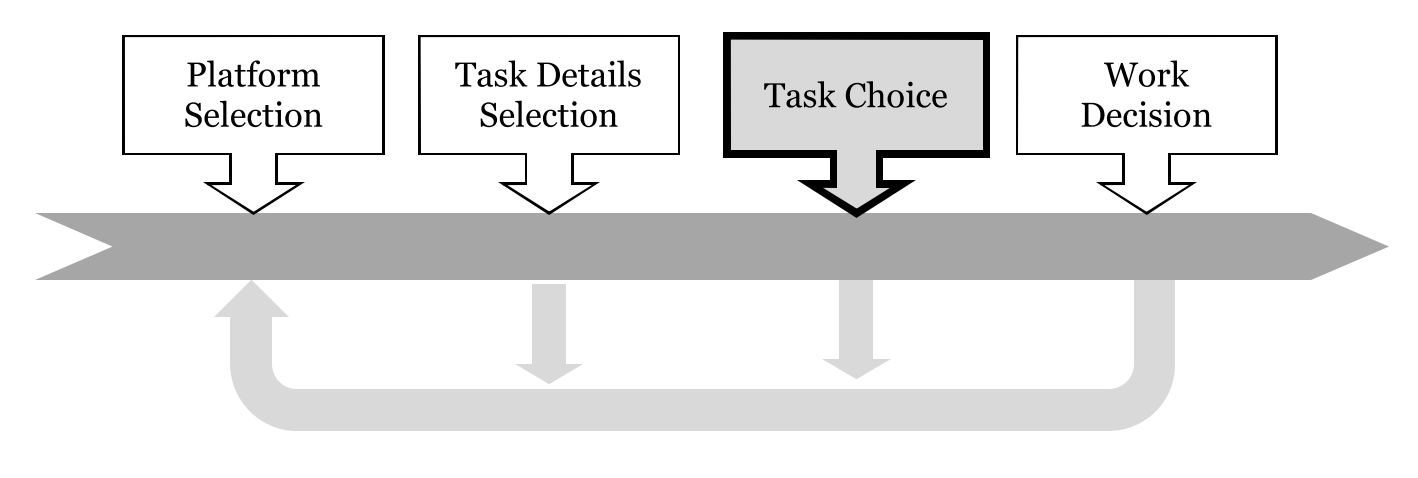
\includegraphics[width=0.5\linewidth]{fig/taskselectionprocess}
	\caption{Micro-tasking workers task selection process \citep{Schulze2012}}
	\label{fig:taskselectionprocess}
\end{figure}

\subsection{Micro-tasking usage}
Micro-tasking and human computation have close ties. In the "Handbook of Human Computation", micro-tasking is strongly present in the \textit{Human Computation for Disaster Response} chapter [\citep{Meier2013}, p. 95-105], as well as in several other parts of the book. In the disaster response chapter, the authors give an overview of how human computation methods, such as paid micro-tasks, could be used to help in major disasters. In 2012, the Philippines was hit by a typhoon called Ruby, devastating large regions. Through CrowdFlower the workers collected over 20 000 tweets related to the typhoon and identified the tweets containing links to either photos or video footage from the damaged areas. The photos and videos in the relevant tweets were tagged and geo-tagged by volunteers if they portrayed evidence of damage. Within 12 hours a dataset of 100 georeferenced images and videos were collected. It resulted in a very detailed crisis map shown in figure \ref{fig:mm-ruby-tweet-crisis-map}. This map was the first official crisis-map based solely on social media content [\citep{Meier2013}, p. 101]. In the aftermath of this crisis, an algorithm was developed to automatically detect tweets that link to photos and videos, which freed more time for the volunteers to georeference and tag more images and videos portraying evidence of damage \citep{Meier2014}.

\begin{figure}[H]
	\centering
	\includegraphics[width=0.6\linewidth]{../../papers/mm-ruby-tweet-crisis-map}
	\caption[Crisis map \citep{Meier2014}]{Typhoon Ruby Crisis map \citep{Meier2014}}
	\label{fig:mm-ruby-tweet-crisis-map}
\end{figure}

The typhoon Ruby crisis map is a good example of exploiting human computation, with crowdsourcing and micro-tasking. It refers to a problem-solving model were a problem or task is outsourced to a distributed group of people by splitting the task or problem into smaller sub-tasks or sub-problems. The sub-tasks is solved by multiple workers independently, often in return for a reward \citep{Sarasua2012}. Thanks to micro-tasking platforms as CrowdFlower and MTurk, it is possible to build a hybrid human-machine system that combines the scalability of computers with the yet unmatched cognitive abilities of the human brain \citep{Difallah2016}.  When analyzing data from MTurk, findings from \cite{Gadiraju2015} indicate rapid growth in micro-task crowdsourcing. With the establishment of micro-task crowdsourcing platforms as MTurk and CrowdFlower, micro-tasking is much more accessible. Micro-tasking practitioners are actively turning towards paid crowdsourcing to solve data-centric tasks that require human input \citep{Gadiraju2015}. Most cases of micro-tasking combine human computation abilities with crowdsourcing.

Companies developing machine-learning algorithms has also seen an advantage in combining fast machine learning algorithms with human computation abilities and crowdsourcing. An example is the team Tomnod\footnote{Tomnod is a team of volunteers who work together to identify important objects and interesting places in satellite images; www.tomnod.com}, who did a project in Australia where they combined human computation, crowdsourcing, and machine learning to locate swimming pools \citep{Kostas2016}. The machine learning algorithm classified polygons where it was likely to be a swimming pool inside. The crowd who participated in finding the swimming pools were only presented with the classified polygons, which minimized the search area and then also the time required finishing the job  \citep{Kostas2016}. Examples of classified polygons are shown in figure \ref{fig:swimmingpoolpolygon3}. The Tomnod team micro-tasked the work. The resulting dataset was then used to train a swimming pool detecting convolutional neural network \citep{Nikki2016}.

\begin{figure}[H]
	\centering
	\includegraphics[width=0.5\linewidth]{../../../../../Desktop/swimmingpoolpolygon3}
	\caption[Swimming pools  \citep{Nikki2016}]{Classified polygons created by the algorithm \citep{Nikki2016}}
	\label{fig:swimmingpoolpolygon3}
\end{figure}

%Micro-tasking has also been used to process queries. In the \cite{Franklin2011} paper they extended a traditional query engine with a small number of operations that requires human input by generating and submitting requests.  They used a micro-tasking platform to get the crowd to answer queries that cannot otherwise be answered. There are especially two cases where human input is needed: a) when the data is unknown or incomplete, b) when there is a need for subjective comparisons. They used auto-generated user interfaces and new query operators that can obtain human input via the interfaces. The \cite{Franklin2011} paper demonstrated that human input can be leveraged to dramatically extend the range of SQL-based query processing. People are good at comparing items, such as how well an image represents a particular concept. Humans are also good at finding relevant information with the help of search engines etc \citep{Franklin2011}. By utilizing these qualities in humans, like they did in \citep{Franklin2011} paper by developing a micro-tasking based implementation of query operations, a huge cost and time sparing potential can be utilized. ''
Another example of micro-tasking usage is the New York Public Library. They use micro-tasking to train computers to recognize building shapes and other data on digitized insurance atlases. %http://buildinginspector.nypl.org/
Humans complete micro-tasks where they check the computer's work and also capture information the computer missed. Individuals contributing checks and fixes building footprints drawn by the computer. The individuals also enter addresses and classify the building footprints using colors. To ensure accuracy, the same footprints are shown to several people. At least three different individuals check the same footprint, and 75\% or more must agree on the footprint for the answer to be approved. 

Most cases of micro-tasking usage exploit the large volume capabilities machines have and the cognitive capabilities of humans \citep{Difallah2016}. 
One of the advantages of micro-tasking platforms like MTurk, Tomnod and CrowdFlower, mentioned by \cite{Meier2013} (p. 99), is the built-in quality control mechanisms that ensure a relatively high quality of output data. They set a review constraint, for instance in a project where they tagged satellite imagery of Somalia. Each unique image was reviewed by at least three different volunteers and only when all three agreed on type and location it was approved. 

\subsection{Building imports in OpenStreetMap using micro-tasking}\label{sec:buildingimport}
%Bygningsimportene til la og ny, her brukte de microtasking til deler av importen
In OpenStreetMap (OSM), at least two large building imports have been successfully achieved using micro-tasking \citep{Erichsen2016}. The first was an import in New York, the second in Los Angeles. Both import teams divided the building dataset into smaller parts to lower the complexity. They used the same python script to create the micro-tasks containing small chunks of building data. Having small chunks of building data made it possible to review and import the data manually into the OSM database \citep{Barth2014d}. In New York, they imported one million buildings partitioned into 5258 micro-tasks \citep{Barth2014d}. In Los Angeles, their dataset contained three million buildings \citep{Sambale2016b}. We have not found how many micro-tasks that were created in total. In both projects, all buildings needed to be quality checked and merged correctly with existing data in OSM. This validation process is done manually in OSM \citep{OSMcommunity2017}. Two massive imports jobs to coordinate. Both building imports used the tasking manager platform (\ref{sec:taskingmanager}) to organize and distribute the micro-tasks [\citep{Barth2014c}, \citep{OSMcommunity2017a}]. The number of buildings in each micro-task varied because the building dataset was partitioned based on already existing subregions which had various building density \citep{Erichsen2016}. 

% When importing new data into OSM, it is likely that it already exists some data there. Data on top of data do not work in OSM, and the new and existing data needs to be appropriately merged. If the existing data contains more detailed information than the new, the community wants to keep the old data, not override it with new, less informative, data. This validation process is done manually in OSM \citep{OSMcommunity2017}. 

A challenge during the New York building import was the underestimated complexity of the import job. It started as a community import where every user in OSM could contribute. Due to the underestimated complexity of the review and upload tasks, and time spent training and supporting new individuals, the team loosely formed a group around the import \citep{Barth2014d}. The company Mapbox participated in the import with experienced team members. The Mapbox members outpaced the local volunteers by a huge factor \citep{Barth2014d}. \cite{Barth2014d} writes that the tasks was not hard but demanded a certain learning curve which meant time someone had to spend teaching new volunteers. Having few experts doing the micro-tasks was evaluated as more effective than involving the whole OSM community. The Los Angeles building import allowed everyone to work on the micro-tasks. They developed the Tasking Manager 2, adding new features to fit their needs. Over 100 volunteers contributed to the import job, working on the micro-tasks posted on the Tasking Manager 2 platform \citep{Sambale2016b}. February 2017, all three million buildings were successfully imported into OSM \citep{OSMcontributors2017}. When examining micro-tasks in both import projects, the overall micro-task in Los Angeles contained fewer buildings than in New York's micro-tasks.  \cite{Erichsen2016} claim that the micro-tasking method is the best-known method when importing large datasets into OSM. This gives a good indication of how useful and functional this method is. 

\subsection{Task complexity}\label{sec:taskcomplexity}
Task complexity has been identified as one of the most important task properties in a variety of fields studying the relationship between human and computers \citep{Yang2016}. The content of the task reflects its complexity, as well as its attributes (i.e., title and description) and visual features (i.e., the layout and color palette) \cite{Yang2016}. \cite{Yang2016} claim that complexity reflects the real mental effort that humans need to put into the completion of tasks. 

Cognitive load theory refers to the total amount of mental effort being used in the working memory. Working memory is determined by the number of information elements that need to be processed simultaneously within a certain amount of time \citep{Barrouillet2007}. A heavy cognitive load can have disadvantageous effects on task completion. Being able to measure and predict task complexity can be highly beneficial for both micro-tasking workers and the requesters \citep{Yang2016}. Too complex tasks can reduce the quality of the results. It is stated that the working memory has a limited capacity of seven plus or minus two elements (or chunks) of information when merely holding information and even fewer (ca. four) when processing information \citep{Leppink2014a}. 

The cognitive load that is imposed by a task is much higher for beginners than for more advanced students \citep{Leppink2014a}. Lack of prior knowledge of how to solve that type of problem forces humans to resort to weak problem-solving strategies \citep{Leppink2014a}. \cite{Gadiraju2015a} looked at how training sections affected the micro-tasking worker's performance. The results showed an improved task performance up to 5\% and task completion time up to 41\% faster than with no training. 

\subsection{Micro-tasking limitations}
Getting enough people to use the micro-tasking platforms is crucial for its success. Most of the platforms mentioned in this chapter give payments to the workers. Another option is to make the platform as a game, which is also shown in this chapter. Creating a micro-tasking platform without payments or gamification factors the page is likely to have a short life, even though the tasking manager, supported by HOT, is an exception to this rule. 

A problem when combining machines and humans is that machines can do their operations in real-time, while humans are unpredictable, they can come and go as they wish. This creates a gap where the micro-tasking platforms cannot guarantee on the task completion time \citep{Difallah2016}. 

The human computation abilities can also be overestimated. During the classification of swimming pools in Australia, the Tomnod team faced some unexpected challenges. As described in section \ref{sec:microtasking}, they used the crowd to classify if a polygon contained a swimming pool or not. When reviewing a random sample from the result, they found an indication that 26\% of polygons that contained a pool were identified as not containing pools by the crowd \citep{Kostas2016}.  Further studies also showed that the guilty part was the crowd, because the algorithm had correctly detected polygons containing pools. In a case where the algorithm was 85\% confident that the polygon contained a pool, only one voted 'yes', six voted 'no, this polygon do not contain a pool'. The solution was to combine the human verdict with the machine's prediction. This example shows that it is important to use the right combination of humans and machines. Tasks that at first seems simple for humans may be more challenging than expected.  Basic object detection using machine learning perform very well when used together with human operations. 

It is important that the tasks added to a micro-tasking platform consider the talents and limitations of human workers \citep{Franklin2011}. By using knowledge provided from OpenStreetMap's usage of the micro-tasking, in \cite{Erichsen2016}, this thesis will examine and hopefully reveal the limitations and talents of human workers when dealing with geospatial micro-tasks. 


